\section{svolgimento delle misure}
La nostra misurazione per essere effettuata si compone di due diverse fasi; una fase di 
calibrazione
dell'apparato; ed una fase in ci vengono 
effettuate la misure 
\subsection{calibrazione }
Per effettuare la calibrazione dell'apparato 
strumentale,siamo andati  a allineare il raggio laser,
il nostro reticolo di diffrazione e lo schermo.
Per osservare sullo schermo un numero
significativo di spot luminosi,essendo $\lambda \gg d$,
attraverso il meccanismo dello specchio abbiamo 
fatto incidere il raggio in maniera radente sul 
nostro reticolo di diffrazione.
Un altro elemento fondamentale della nostra 
calibrazione è la determinazione dello
zero.
La quota dello zero è stata determinata
prendendo il punto intermedio tra il fascio 
diretto,ovvero la parte non riflessa dal calibro,osservata 
in assenza di calibro,
e lo spot corrisponde alla riflessione
speculare sul calibro, ovvero il primo punto più luminoso
osservato eccetto il fascio non riflesso,osservato una
volta reinserito il calibro.
\subsection{procedimento e misure}
Dalla conoscenza del passo reticolare $d$ e
dalla  differenza di cammino ottico,$\Delta L$
di un'onda piana incidente con un angolo $\theta_i$\footnote{gli angoli $\theta_d$ e $\theta_i$ sono misurati rispetto alla normale al reticolo.}
possiamo ricavare 
\smallskip
\begin{equation}\label{eq:delta L}
\Delta L = d \cdot (sin \theta_i - sin \theta_d)
\end{equation}
\smallskip
dove $\theta_d$ è l'angolo di riflessione 
riferito alla normale del reticolo.
I punti di massima intensità della nostra radiazione 
devono corrispondere a punti per i quali 
la differenza di cammino ottico 
$\Delta L$ corrisponde a multipli della 
lunghezza d'onda $\lambda$
ottenendo pertanto 
\smallskip

\begin{equation}\label{eq:delta L2}
m \lambda = d \cdot (sin \theta_i - sin \theta_d) \qquad m\in N.
\end{equation}
\smallskip
Dalla misura della posizione angolare dei nostri
massimi e dalla \textbf{equazione \ref{eq:delta L2}}
possiamo ricavare una stima di $\lambda$.
Per migliorare la significatività della 
misura,essendo visibili più
spot di massimo,
abbiamo eseguito un fit lineare
di $m$ ,numero corrispondente al n-esimo
spot di massimo, e del corrispondente
$ sin \theta_d$;
impiegando la relazione 
\smallskip
$$ sin \theta_d =-\frac{\lambda}{d}m+sin \theta_i.$$
\smallskip
\\
Per effettuare le nostre misure abbiamo
impiegato la tecnica descritta precedentemente.
Data la strumentazione impiegata 
si ha un passo reticolare $d=1\text{ }[mm]$ 
dove abbiamo assunto trascurabile l'errore dovuto alla
tacca del calibro;%sarebbe tile fare considerazioni sll errore da associare al calibro dovrebbe rispettare la normativa UNI - ISO 3599 Vernier callipers reading to 0,1 and 0,05 mm, ma non ho avto il tempo di gardarla ad ora



dalle seguenti relazioni abbiamo ricavato $sen \theta_d$ 
\smallskip 
\begin{equation} \label{sen rif}
sen \theta_n = {(1+\frac{{h_n}^2}{{D}^2}})^{-1/2}\qquad \text{e}\qquad \theta_d= \pi/2 - \theta_n
\end{equation}

\smallskip
dove $h_n$ è l'altezza sullo schermo del n-simo 
massimo rispetto allo zero ottenuto
col calibramento,
$D$ è la distanza tra il punto di incidenza 
della radiazione emessa e lo schermo di diffrazione.
Per l'incertezza associata a tali misure
poiché $d\gg \lambda_{attesa}$ necessitiamo che il raggio laser abbia
incidenza  pressoché radente.
A seguito di tale orientazione si osserva che il
punto di incidenza 
presenta un estensione non trascurabile;
si è infatti misurato $[D_{min};D_{max}]= [206;212] [cm]$ 
assumendo come valore di $D= 209 [cm]$, il valore della 
semiampiezza dell'intervallo  $\Delta D = 3 [cm]$.
Analogo procedimento è stato effettuato per determinare $h_n$ degli spot
di massimo.

Si riportano i dati così ottenuti in \begin{table}[hb]
 \centering
 \begin{tabular}{|c|c|c|}
 \hline
 \hline
  Ordine $m$ & Distanza $h$ [cm] & $\sigma_h [cm]$ \\
  \hline
  zero di riferimento rispetto al fascio diretto	&	$6.9$	&	$0.1$\\
  \hline
  $1$  & $10.15$ & $0.10$ \\
  $2$  & $12.60$ & $0.15$ \\
  $3$  & $14.65$ & $0.15$ \\
  $4$  & $16.45$ & $0.15$ \\
  $5$  & $18.05$ & $0.15$ \\
  $6$  & $19.50$ & $0.15$ \\
  $7$  & $20.90$ & $0.2$ \\
  $8$  & $22.25$ & $0.25$ \\
  $9$  & $23.45$ & $0.15$ \\
  $10$ & $24.75$ & $0.15$ \\
  $11$ & $25.75$ & $0.20$ \\
  $12$ & $26.85$ & $0.20$ \\
  $13$ & $27.85$ & $0.20$\\
  $14$ & $28.85$ & $0.25$ \\
  $15$ & $29.90$ & $0.30$ \\
  $16$ & $30.85$ & $0.35$ \\
  $17$ & $31.70$ & $0.30$ \\
  $18$ & $32.55$ & $0.35$ \\
  $19$ & $33.50$ &	$0.40$\\
  \hline
 \end{tabular}
 \caption{Posizione massimi frange di interferenza per diffrazione su calibro.
Essendo la lettura fatta  col metro ed essendo possibile osservare la
mezza tacca abbiamo associato una sensibilità di $0.05[cm]$ 
superiore alla sensibilità nominale dello strumento.
I valori eccetto quello dello zero di riferimento sono dati
rispetto allo zero di riferimento.}
	\label{tab:Ha-Na}
\end{table}
 \tabella{tab:Ha-Na}.

Impiegando i dati \tabella{tab:Ha-Na} 
otteniamo come risultato del fit $sin \theta_d = a \cdot m + b$,
\begin{figure} [!h]
	\centering
	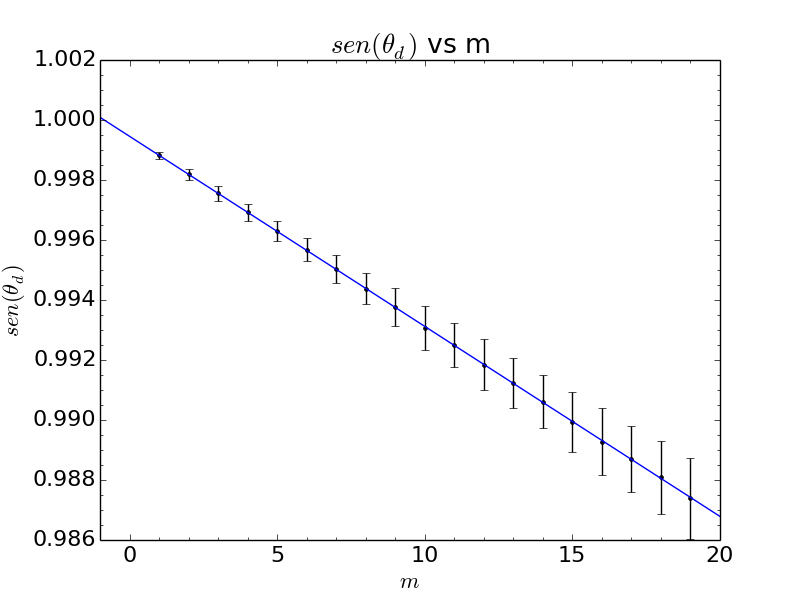
\includegraphics[width=0.9\textwidth]{./pictures/fitprova}
	\caption{Fit di$sin \theta_d = a \cdot m + b$ .}
	\label{fig:fit}
\end{figure}
riportato in \figura{fig:fit} 
\smallskip
$$a=(634	\pm	1	)\cdot 10^(-6)	\qquad	b=(		\pm		)	\qquad \text{ed un relativo}\qquad \frac{\chi^2}{ndof}\sim $$
\smallskip
dal quale otteniamo \smallskip\begin{equation}
\lambda=-a \cdot d = (634	 \pm 1	)[nm] \\
\theta_i=arcsin(b)=
\end{equation}
a fronte di $ \lambda_{atteso}=633 [nm]$